\chapter{Módulo hardware}
<<<<<<< HEAD
\label{cap:hard}


En esta parte nos centraremos en profundizar en las parte más tangible del proyecto, introduciendo la electrónica y 
mecánica del mismo.

Es importante destacar que gracias a las  diferentes plataformas de hardware libre he podido reducir en gran parte el alcance del proyecto, pudiéndome  centrar en implementar las funcionalidades y no tanto en montar todo el marco de trabajo necesario para llegar a ello. 

Tenemos presentes las herramientas de última generación, que están teniendo un gran auge y aceptación 
en la comunidad DIY, como lo son las \textbf{impresoras en 3D} o las \textbf{cortadoras láser}, que agilizan la mecanización y fabricación de las partes mecánicas.


\section{Análisis}

Después de las reuniones con el cliente y el estudio del dominio puedo llegar a extraer los requisitos que debe satisfacer el dispositivo para el objetivo propuesto. Dichos requisitos se desglosan a continuación.

\subsection{Requisitos funcionales}

\begin{itemize}
	\item \textbf{RF-1.}: Controlar motor paso a paso:
	\begin{itemize}
		\item \textbf{RF-1.1.}: Controlar la dirección.
		\item \textbf{RF-1.2.}: Controlar velocidad.
		\item \textbf{RF-1.3.}: Controlar microstepping, para conseguir la máxima resolución en los pasos. \cite{micros}
	\end{itemize} 	
		\item \textbf{RF-2.}: Mostrar información del sistema mediante una pantalla LCD.
		\item \textbf{RF-3.}: Modificar parámetros de forma manual.
	\begin{itemize}
		\item \textbf{RF-3.1.}: Modificar velocidad.
		\item \textbf{RF-3.2.}: Modificar mover \texttt{n} pasos por pulsación.
	\end{itemize}	
	\item \textbf{RF-4.}:Ejecutar funciones de movimiento del motor desde una botonera o control manual.
		\begin{itemize}
			\item \textbf{RF-4.1.}: Ejecutar función de movimiento continuo en la dirección deseada.
			\item \textbf{RF-4.2.}: Ejecutar función de movimiento (\texttt{n} pasos) en la dirección deseada. 
		\end{itemize}
	\item \textbf{RF-5.}: Monitorizar temperatura y mostrar aviso cuando se detecte un cambio.
	\item \textbf{RF-6.}: Controlar límites físicos en el desplazamiento de las partes mecánicas del enfocador.  	
\end{itemize}

\subsection{Requisitos no funcionales}

\begin{itemize}
	\item \textbf{RNF1.}: El movimiento del motor debe tener una precisión alta y una suavidad adecuada. 
	\item \textbf{RNF2.}: Los controles deben ser intuitivos y responder de forma interactiva. 
	\item \textbf{RNF3.}: La pantalla LCD no debe tener excesiva iluminación para conservar la oscuridad.
	\item \textbf{RNF4.}: Fácil instalación y trasporte.
	\item \textbf{RNF5.}: Dispositivo robusto y tolerante a condiciones adversas, sesiones de trabajo prolongadas, así como posibles golpes y movimientos.
	\item \textbf{RNF6.}: Bajo consumo, dado que puede ser alimentado por baterías.
\end{itemize}

\section{Planificación}

\begin{itemize}
	\item \textbf{Fase 0:} \textbf{Planteamiento del problema}.
	\begin{itemize}
		\item \textbf{Reunión inicial con el cliente}: Donde se propone la idea y los puntos clave del proyecto. 
		\item \textbf{Investigar la temática}: Buscar enfocadores comerciales, ver su funcionalidad y posibles nuevas funcionalidades.
		\item \textbf{Segunda reunión con cliente}: Se proponen las funcionalidades más interesantes y se compara con los dispositivos comerciales estudiados, el cliente corrobora que las funciones resultan más o menos interesantes desde su punto de vista como astrónomo amateur.
	\end{itemize}
	\item \textbf{Fase 1:} \textbf{Investigar tecnologías implicadas}.
	\begin{itemize}
		\item \textbf{Estudiar tecnologías que se emplearán}, para ello se estudian las diferentes plataformas de hardware libre, comparando a grandes rasgos sus puntos fuertes, limitaciones, así como otros aspectos como precio, soporte por la comunidad, componentes y repuestos.
		
		\item \textbf{Buscar componentes} a utilizar y comparar precios con los diferentes proveedores.
	\end{itemize}
	\item \textbf{Fase 2:} \textbf{Análisis y diseño}.
	\begin{itemize}
		\item Redactar formalmente los \textbf{requisitos} del sistema. 
		\item Realizar \textbf{esquemáticos} de la electrónica. 
		\item Realizar \textbf{diseños} para el corte de la caja exterior.
	\end{itemize}
	\item \textbf{Fase 3:} \textbf{Implementación}.
	\begin{itemize}
		\item \textbf{Montaje versión 0} del dispositivo usando placas de prototipado y cables.		
		\item \textbf{Corte de piezas} para construir la carcasa del dispositivo. 
		\item \textbf{Soldadura de la PCB}, con todos los componentes, 
		\item \textbf{Montaje prototipo 1}, versión 1, haciendo uso de la caja y la placa PCB. 
	\end{itemize}
	\item \textbf{Fase 4:} \textbf{Pruebas}.
	\begin{itemize}
		\item \textbf{Pruebas de los componentes}, asegurando que no tienen defectos de fábrica.
		\item \textbf{Pruebas prototipo versión 0}.
		\item \textbf{Pruebas prototipo versión 1}.
	\end{itemize} 
\end{itemize}


\subsection{Mockup}


Un primer boceto que se realiza del sistema con los requisitos anteriores es el mostrado en la figura~\ref{fig:diagrama_ardufocuser}.

\begin{figure}[h]
\centering
\includegraphics[width=1\linewidth]{../images/diagrama_ardufocuser}
\caption[Mockup del dispositivo hardware]{Diseño parte externa del dispositivo, donde podemos ver los diferentes controles.}
=======

\bigskip
En esta parte me dedicaré a profundizar en las parte más tangible del proyecto, introduciendo así en la electrónica, 
mecánica.

\bigskip
Es importante destacar que gracias alas  diferentes plataformas de hardware libre he podido reducir en gran parte el alcance del proyecto, pudiendo así centrarme en implementar las funcionalidades y no tanto en montar todo el marco de trabajo necesario para llegar a ello. 

\bigskip
Teniendo presentes las  herramientas de última generación, que están teniendo un gran auge y aceptación 
en la comunidad DIY \cite{DIY} "hágalo usted mismo", como lo son las \textbf{impresoras en 3D} o las \textbf{cortadoras láser}, que agilizan la mecanización y fabricación de las partes mecánicas.

\section{Fases}

\begin{itemize}
	\item \textbf{Fase 0:} Planteamiento del problema.
	\item \textbf{Fase 1:} Investigar tecnologías implicadas.
	\item \textbf{Fase 2:} Análisis y diseño.
	\item \textbf{Fase 3:} Implementación.
	\item \textbf{Fase 4:} Pruebas.
\end{itemize}


\section{Estimación de tiempos}



\section{Requisitos sistema hardware}

EL requisito principal del sistema hardware es actuar sobre la \textbf{ruleta de ajuste del foco} que incorpora el \textbf{ocular del telescopio}. 

Este movimiento tiene que ser perfectamente controlado, con una precisión alta y una suavidad adecuada. 

El movimiento debe responder a las ordenes, que proporcione directamente el usuario por medio de un \textbf{control manual} o bien las ordenes en forma de comandos  que comunique la rutina de enfoque automático que se ejecute.

El control manual permite girar el enfocador en ambos sentidos de dos modos diferentes:
    1. Movimiento continuo, hasta llegar al límite físico.
    2. Movimiento de n pasos.

Modificar la velocidad dentro de un rango válido.
Modificar el número n de pasos por pulsación. 
Establecer posición actual, como posición de foco válido dada la temperatura actual. 
 
Mediante comandos podemos acceder y modificar todos los estados del sistema, respondiendo con un mensaje que informa del cambio producido. 

Para emular la característica de compensación térmica, incorpora un sensor térmico, que permita avisar al usuario de cambios considerables en la temperatura de la óptica, siendo una alarma para revisar el valor del enfoque.  

Debe existir una pantalla que proporcione la máxima información del sistema, (posición de enfoque, velocidad seleccionada, temperatura).


Un primer boceto que se realiza del sistema con los requisitos anteriores es el siguiente:

\begin{figure}[h]
\centering
\includegraphics[width=0.7\linewidth]{../images/diagrama_ardufocuser}
\caption{}
>>>>>>> c9f08dfe66521d4f0dba18e652f93a6a37a333aa
\label{fig:diagrama_ardufocuser}
\end{figure}


<<<<<<< HEAD
\section{Diseño sistema hardware y electrónica: arquiectura del sistema}

Para la elaboración y diseño del sistema hardware hemos seleccionado distintos componentes que hemos agrupado en los siguientes módulos:

\begin{itemize}
 \item Núcleo: Arduino
 \item Módulo de motores
 \item Módulo de pantalla
 \item Módulo de sensores
 \item Módulo de control manual
\end{itemize}

Estos módulos se describen en las siguientes secciones.

En la figura~\ref{fig:diagramaHardware} mostramos un esquemático en el que se integran los distintos componentes hardware.

\begin{figure}[h]
	\centering
	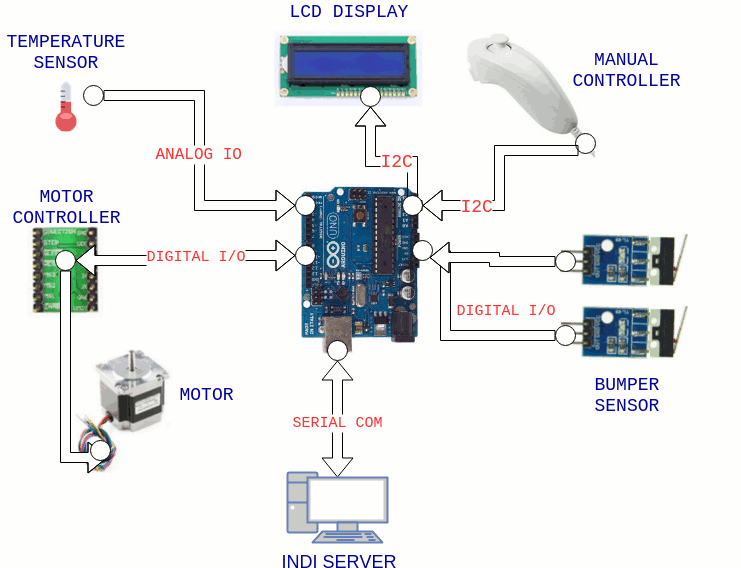
\includegraphics[width=1\linewidth]{../images/diagramaHardware}
	\caption[Diagrama general, sistema hardware]{\textbf{Diagrama general, sistema hardware.} En el diagrama podemos ver los elementos que intervienen y de forma simplificada la relación que existe entre ellos.}
	\label{fig:diagramaHardware}
\end{figure}



\subsection{Núcleo: Arduino}
Para el diseño de la electrónica, partimos como base de una placa de prototipo \textbf{Arduino} \cite{ARDUINO}.

El hardware consiste en una placa de circuito impreso con un microcontrolador, usualmente \textbf{Atmel AVR} \cite{Atmel}, junto con  puertos digitales y analógicos para entrada/salida.

Las características principales de las placas Arduino, que pueden servirnos para decidirnos entre un tipo de placa u otro son las siguientes:
=======
\section{Diseño sistema hardware y electrónica}

Las entrada al sistema hardware de enfoque, proviene de cuatro fuentes.

\begin{enumerate}
\item Los sensores inherentes al dispositivo.
\item Variables de configuración o estados de la sesión anterior. 
\item Controles manuales, ya sean botoneras o potenciómetros.
\item Controles remotos provenientes, que llegan al dispositivo en forma de comandos, por el puerto serie.
\end{enumerate}

Por tanto el sistema hardware, se descompone en los siguiente módulos.

\begin{itemize}

\item Módulo para el control de motores, encargado de actuar sobre el motor, de forma precisa.

Controlar variables y estados tales como, posición actual, velocidad, aceleración, sentido de giro y respetando los módulos de sensores y control. 

\item Módulo de sensores. Se ocupa de manejar la información proveniente de sensores externos, tales como sensores finales de recorrido, sensor de temperatura.

Controlando estados, presencia de un tope que limite el movimiento en uno de los sentidos, temperatura de último enfoque y actual.

\item Módulo control manual, se encarga de leer los diferentes botones y potenciómetros, con los que el usuario puede manejar directamente el dispositivo.
Tenemos estados para cada uno de los botones y los comunica al módulo de motores, cambia la configuración o lo comunica por puerto serie y/o módulo de visualización LCD.

\item Módulo de control remoto, su trabajo es estar a la escucha de los posibles comandos que puedan llegas por puerto serie y comunicarlo al modulo que corresponda. 

\item Modulo de configuración y almacenamiento de sesión, se encarga de manejar todas las variables de configuración, así como almacenarlos en EEPROM, para que se mantengan de forma persistente para la próxima sesión de trabajo

\end{itemize}




\section{Implementación dispositivo hardware}

\subsection{Framework Arduino}
Para el diseño de la electrónica, partimos como base de una placa de prototipo Arduino.

\bigskip
El hardware consiste en una placa de circuito impreso con un microcontrolador, usualmente \textbf{Atmel AVR} \cite{Atmel}, junto con  puertos digitales y analógicos para entrada/salida.

\bigskip
Por otro lado, el software consiste en un entorno de desarrollo (IDE) basado en \textbf{Processing} \cite{Process}  y lenguaje de programación basado en \textbf{Wiring}, así como en el cargador de arranque (bootloader) que es ejecutado en la placa.

Características principales de las placas Arduino, que pueden servirnos para decidirnos entre un tipo de placa u otro.
>>>>>>> c9f08dfe66521d4f0dba18e652f93a6a37a333aa

\begin{itemize}
	\item \textbf{Microcontrolador}, por su arquitectura y su frecuencia de reloj.
	\item \textbf {Tamaño de las memorias},
	\begin{itemize}
<<<<<<< HEAD
		\item{\textbf{Flash}} (espacio del programa) es donde Arduino almacena el \textbf{sketch}. Esta memoria es no volátil y su tamaño oscila entre los 16 kilobytes.
		
		\item{\textbf{SRAM}} Memoria estática de acceso aleatorio, de tipo volátil. Es el espacio donde los sketches (programas) almacenan y manipulan variables al ejecutarse. La información guardada en esta memoria será eliminada cuando Arduino pierda la alimentación. Esta memoria es de uso exclusivo para el programa en ejecución. Su tamaño oscila en torno a los 1024 bytes.
		
		\item{\textbf{EEPROM}} es un espacio de memoria que puede ser utilizado por los programadores para almacenar información a largo plazo. Este tipo de memoria es no volátil, por lo que los datos guardados en ella permanecerán aunque Arduino pierda la alimentación. Permite almacenar configuraciones de la sesión. Es importante resaltar quee tiene un número de escrituras muy limitado por lo cual no se puede usar de forma extensiva. Su tamaño oscila en torno a los 512 bytes.
=======
		
		\item{Flash} (espacio del programa) es donde Arduino almacena el \textbf{sketch}\footnote{Un sketch es el nombre que usa Arduino para un programa.}. Esta memoria es no volátil y su tamaño oscila entre los 16 kilobytes.
		
		\item{SRAM} Static Random Access Memory ó memoria estática de acceso aleatorio,  es de tipo volátil, es el espacio donde los sketches (programas) almacenan y manipulan variables al ejecutarse. La información guardada en esta memoria será eliminada cuando Arduino pierda la alimentación. Esta memoria es de uso exclusivo para el programa en ejecución. Su tamaño oscila entre los 1024 bytes.
		
		\item{EEPROM} es un espacio de memoria que puede ser utilizado por los programadores para almacenar información a largo plazo. Este tipo de memoria es no volátil, por lo que los datos guardados en ella permanecerán aunque Arduino pierda la alimentación. Permite almacenar configuraciones de la sesión, he de decir que tiene un número de escrituras muy limitado por lo cual no se puede usar de forma extensiva. Su tamaño oscila entre los 512 bytes.
>>>>>>> c9f08dfe66521d4f0dba18e652f93a6a37a333aa
		
	\end{itemize}
	\item \textbf {Puertos de entrada y salida I/O}. Son los puertos que disponemos para comunicarnos con los periféricos, ya sean sensores o actuadores. 
	\begin{itemize}
<<<<<<< HEAD
		\item \textbf{Digitales}: Estos \textbf{pines}, tal como podemos intuir trabajan con señales digitales de 5V, (estados LOW y HIGH), existiendo un tipo de especial de ellos denominados \textbf{PWM}, que permiten ``emular" señales analógicas. Otro punto a tener en cuenta es el número de pines que permiten ejecutar \textbf{interrupciones hardware}. 
		
		\item \textbf{Analógicos}: Permiten lectura de valores analógicos que se encuentren el la escala de 0V a 5V. Las entradas analógicas disponen de 10 bits de resolución, lo que proporciona 1024 niveles digitales, lo que a 5V supone una precisión de la medición de +-2,44mV. 
=======
		\item{Digitales} Estos \textbf{pines}\footnote{patilla metálica de un conector multipolar.}, tal como podemos intuir trabajan con señales digitales de 5V, (estados LOW y HIGH), existiendo un tipo de especial de ellos denominados \textbf{PWM}\footnote{señal de modulación por ancho de pulso}, que permite ``emular", señales analógicas. \newline
		Otro punto a tener en cuenta es el número de pines que permiten ejecutar  \textbf{interrupciones hardware}. 
		
		\item{Analógicos}, permiten lectura de valores analógicos que se encuentren el la escala de 0V a 5V, las entradas analógicas disponen de 10 bits de resolución, lo que proporciona 1024 niveles digitales, lo que a 5V supone una precisión de la medición de +-2,44mV. 
		
>>>>>>> c9f08dfe66521d4f0dba18e652f93a6a37a333aa
	\end{itemize}
	
	\item \textbf{Otros factores}
	\begin{itemize}
<<<<<<< HEAD
		\item \textbf{Factores de forma}: Características como las dimensiones, el peso, la forma.
		\item \textbf{Conectores auxiliares}: Tamaño y forma de los conectores USB, ya sea de Tipo A, Tipo B o mini-USB. 
		\item \textbf{Consumo}: Muy importante si alimentamos la placa con  baterías. 
=======
		\item \textbf{Factores de forma}, características como las dimensiones, el peso, la forma.
		\item \textbf{Conectores auxiliares}, Tamaño y forma de los conectores USB, ya sea de Tipo A, Tipo B o mini-USB. 
		\item \textbf{Consumo}, muy importante si alimentamos la placa con  baterías. 
		
>>>>>>> c9f08dfe66521d4f0dba18e652f93a6a37a333aa
	\end{itemize}	
\end{itemize}


\begin{figure}[h]
<<<<<<< HEAD
	\centering
	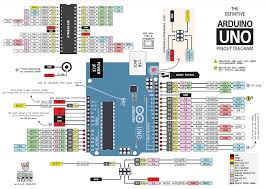
\includegraphics[width=1\linewidth]{../images/arduino_data}
	\caption[Diagrama de pines de Arduino]{\textbf{Diagrama de pines de Arduino}, muestra los diferentes pines de entrada/salida de la placa Arduino UNO, así como sus conexiones con el microcontrolador. También podemos ver los pines de alimentación a 5V y 3V3. \textbf{Fuente: }\cite{ARDUINO}}
	\label{fig:arduino_data}
\end{figure}

Para este proyecto hemos seleccionado la placa \textbf{Arduino UNO} (figura~\ref{fig:arduino_data}) en base a los siguientes criterios:

\begin{itemize}
	\setlength\itemsep{0em}
	\item \textbf{Precio reducido}, que oscila en torno a los los 20 \euro.
	\item \textbf{Potencia del procesador y memoria}, suficiente para soportar el firmware a implementar.
	\item \textbf{Conector USB tipo B}, al ser de buen tamaño, hace la conexión robusta (importante en telescopios donde existe movimiento o posibles tensiones en los cables).
	\item \textbf{Número de pines}, suficiente para conectar todos los periféricos previstos.
	\item \textbf{Características especiales}, (PWM y interrupciones hardware). 
	\item \textbf{Comunicación I2C}. 
\end{itemize}

\subsection{Módulo de motores}

Para permitir el control del motor de un paso a paso, usaremos un Pololu A4988 \cite{pololu} (figura~\ref{fig:pololu}). Las características más reseñables de tal controlador y que los hacen destacar frente a sus competidores son las siguientes:

\begin{itemize}
	\item{Interfaz simple} para controlar pasos y dirección.
	\item{Cinco resoluciones de paso diferentes}, paso completo, $1/2$ paso, $1/4$ de paso, $1/8$ de paso y $1/16$ de paso. 
	\item{Control de corriente} de paso ajustable.
	\item{Protecciones} contra sobretensiones y sobrecalentamientos.
=======
\centering
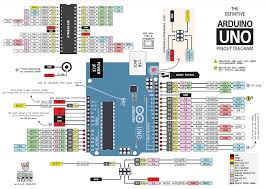
\includegraphics[width=0.8\linewidth]{../images/arduino_data}
\caption{Arduino Pinout Diagram}
\label{fig:arduino_data}
\end{figure}


\newpage

Me decido por Arduino UNO en base a los siguientes criterios:

\begin{itemize}
	\item{Precio reducido}, que oscila entre los 20 \euro
	\item{Potencia del procesador y menoría}, suficiente para soportar el firmware.
	\item{Conector USB tipo B}, al ser de buen tamaño, hace la conexión robusta.
	\item{Número de pines} suficiente para conectar todos los periféricos.
	\item{Características especiales}, (PWM y interrupciones hardware). 
	\item{I2C} compatible. 
\end{itemize}


\subsection{Módulo de motores}

Para permitir el control del motor de un paso a paso,  Pololu A4988 \cite{pololu},
las características más reseñables de tal controlador y que los hacen destacar frente a sus competidores.

\begin{itemize}
	\item{} Interfaz simple para controlar pasos y dirección.
	\item{} Cinco resoluciones de paso diferentes, paso completo, medio paso, cuarto de paso, octavo de paso, dieciseisava parte de paso. 
	\item{} Control de corriente de paso ajustable.
	\item{} Protecciones contra sobretensiones y sobrecalentamientos.
>>>>>>> c9f08dfe66521d4f0dba18e652f93a6a37a333aa
\end{itemize}


\begin{figure}[h]
<<<<<<< HEAD
	\centering
	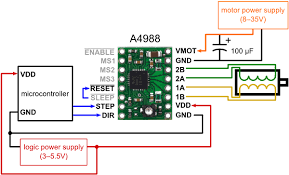
\includegraphics[width=0.8\linewidth]{../images/pinout_pololu}
	\caption[Diagrama Pololu A4988]{\textbf{Pololu A4988} - Vista del controlador de motor paso a paso utilizado. Podemos observar las diferentes conexiones, puertos de control (STEP y DIR), alimentación del controlador (VDD), alimentación del motor (VMOT), salidas para el motor (1A, 1B, 2A, 2B) y pines para ajuste de la resolución de pasos (MS1, MS2, MS3) \textbf{Fuente:} \cite{pololu} }
	\label{fig:pololu}
\end{figure}

El motor empleado para nuestro sistema es un motor paso a paso \textbf{NEMA 17} / 3.2Kg/cm, de uso muy habitual, en el montaje de impresoras 3D. Sus características principales son las siguientes:

\begin{itemize}
	
	\item \textbf{Tamaño:} 42.3x48mm (sin incluir el eje) (NEMA 17)
	\item \textbf{Peso:} 350 gramos (13 oz)
	\item \textbf{Diámetro del eje:} 5 mm "D"
	\item \textbf{Longitud del eje:} 25 mm
	\item \textbf{Pasos por vuelta:} 200 (1.8\degree/paso)
	\item \textbf{Corriente:}  1.2 Amperios por bobinado
	\item \textbf{Tensión:} 12 V
	\item \textbf{Resistencia:} 3.3 Ohm por bobina
	\item \textbf{Torque:} 3.2 kg/cm (44 oz-in)
	\item \textbf{Inductancia:} 2.8 mH por bobina 
=======
\centering
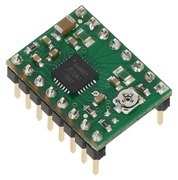
\includegraphics[width=0.3\linewidth]{../images/pololu}
\caption{Pololu A4988 Stepper Motor Driver Carrier}
\label{fig:pololu}
\end{figure}

\newpage

El motor empleado es un Motor paso a paso NEMA 17 / 3.2Kg/cm, de uso muy habitual, 
en el montaje de impresoras 3D,  

\bigskip
Sus características son las siguientes.

\begin{itemize}
	\item{Tamaño:} 42.3x48mm, sin incluir el eje (NEMA 17)
	\item{Peso:} 350 gramos (13 oz)
	\item{Diámetro del eje:} 5 mm "D"
	\item{Longitud del eje:} 25 mm
	\item{Pasos por vuelta:} 200 (1,8º/paso)
	\item{Corriente:}  1.2 Amperios por bobinado
	\item{Tensión:} 4 V
	\item{Resistencia:} 3.3 Ohm por bobina
	\item{Torque:} 3.2 kg/cm (44 oz-in)
	\item{Inductancia:} 2.8 mH por bobina 
>>>>>>> c9f08dfe66521d4f0dba18e652f93a6a37a333aa
\end{itemize}

\subsection{Módulo de pantalla}

<<<<<<< HEAD
Para visualizar los estados del sistema fácilmente, se incorporará una pequeña pantalla LCD. Uno de los displays LCD más corrientes son los alfanuméricos de 16x2 o 16x4 caracteres.

Para su utilización en un principio se estima controlarla mediante los pines digitales usando 4 señales digitales D7, D6, D5, y D4, junto con dos pines adicionales de control tal y como se puede ver ver en las figuras~\ref{circuito1} y \ref{circuito2} del apéndice~\ref{ap:diagramas}.


En una fase de rediseño optimizamos el circuito incorporando un \textbf{interfaz I2C}, reduciendo las señales a solo dos (figura~\ref{fig:lcd_i2c}). 

\begin{figure}[h]
	\centering
	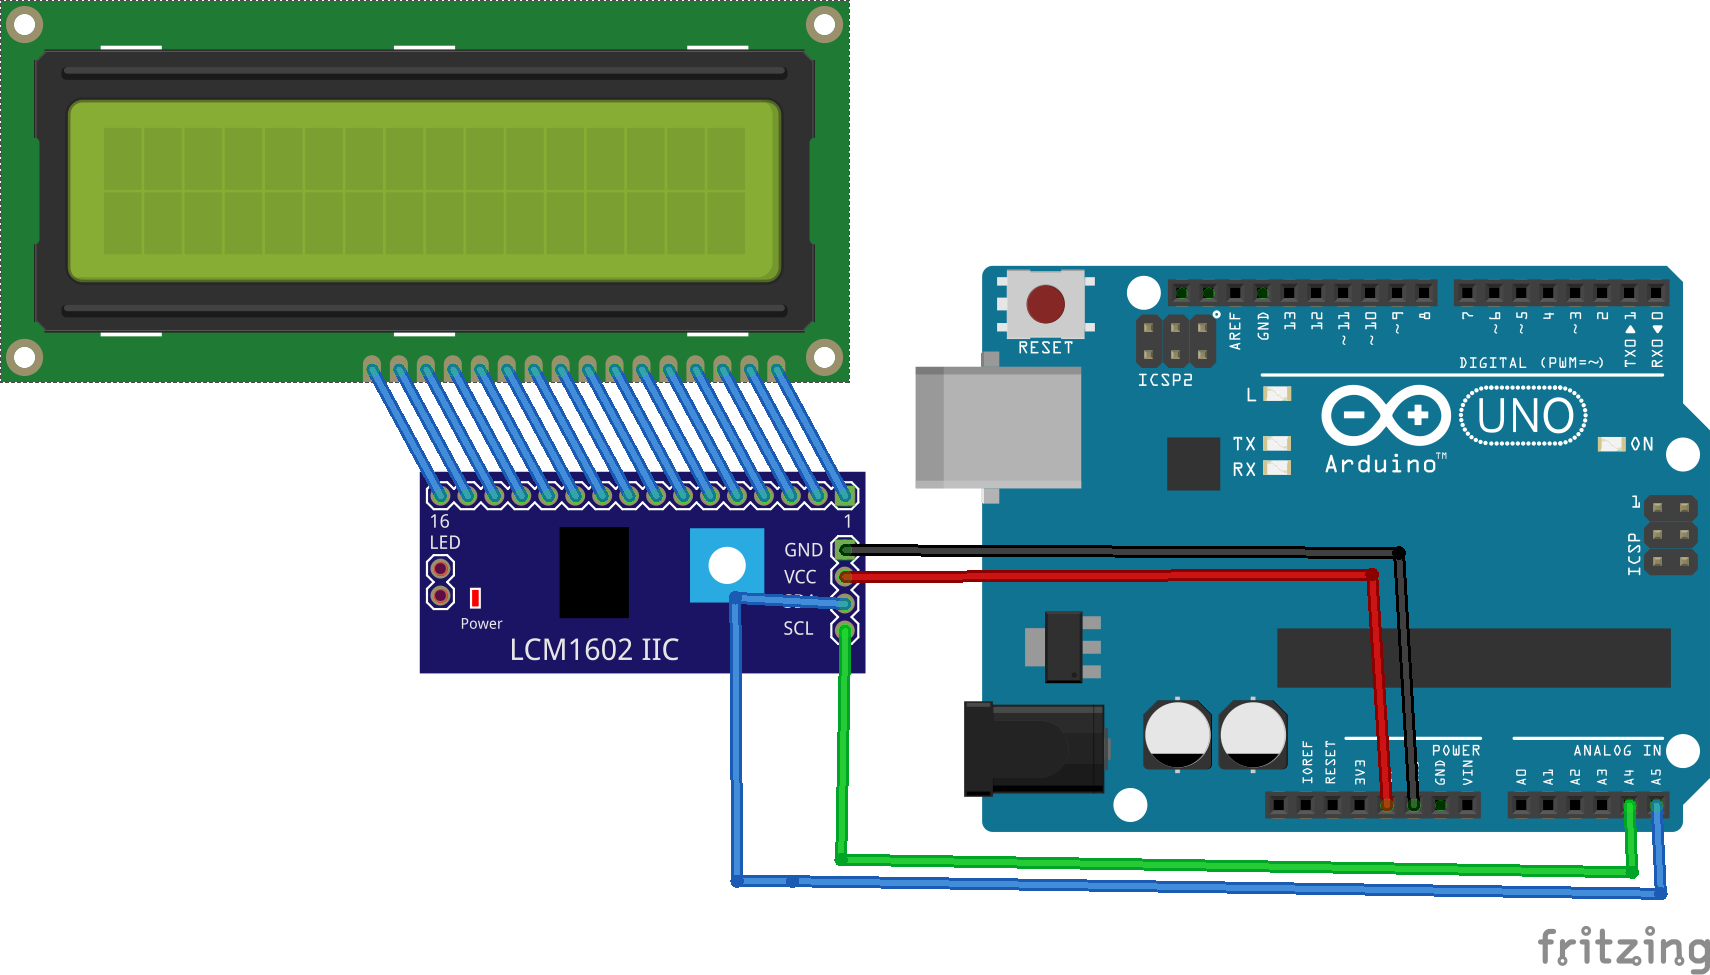
\includegraphics[width=0.7\linewidth]{../images/lcd_i2c}
	\caption[Diagrama conexión pantalla LCD con interfaz I2C]{Diagrama conexión pantalla LCD con interfaz I2C}
	\label{fig:lcd_i2c}
\end{figure}


\subsection{Módulo de sensores}
=======
Para visualizar los estados del sistema fácilmente, el sistema incorpora una pequeña pantalla LCD. 

Los más corrientes son los display LCD, de 16x2 o 16x4.

Para su utilización en un principio se estima controlarla mediante los pines digitales usando 4 señales digitales D7, D6, D5, y D4, junto con dos pines adicionales de control. Como podemos ver en los primeros diagramas.

En una fase de rediseño optimizamos el circuito incorporando una interfaz I2C \cite{I2C}, reduciendo las señales a solo dos. 


\subsection{Módulo sensores}
>>>>>>> c9f08dfe66521d4f0dba18e652f93a6a37a333aa

El dispositivo incorpora dos tipos de sensores:

\begin{itemize}
<<<<<<< HEAD
	\item \textbf{Sensor térmico:} Hacemos uso de un sensor LM35 \cite{LM35}. Es un sensor de temperatura con una precisión calibrada de 1 \grad C. Su rango de medición abarca desde -55\grad C hasta 150 \grad C. La salida es lineal y cada grado Celsius equivale a 10 mV.
	
	
	En una fase de rediseño se reemplaza el sensor por uno del tipo DHT11 \cite{dth11}, que mide temperatura en el rango -10 \grad C y 50\grad C. Adicionalmente tambien mide humedad, en un rango del 20\% al 95\% (figura~\ref{fig:dht11}). Usa un protocolo de un solo hilo digital, (1-wire). 
	
	
	\begin{figure}[h]
		\centering
		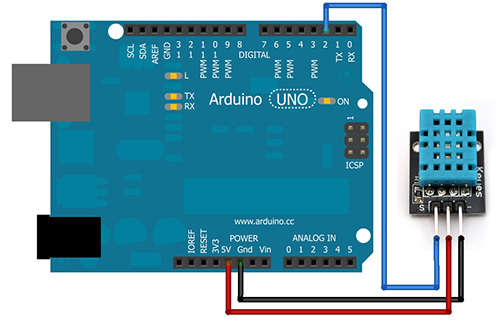
\includegraphics[width=0.5\linewidth]{../images/dht11}
		\caption[Diagrama sensor de temperatura y humedad DHT11]{Diagrama de conexión del sensor de temperatura y humedad DHT11}
		\label{fig:dht11}
	\end{figure}
	
	\item \textbf{Endstop sensor}, o contactos fines de carrera. Son interruptores del tipo todo o nada, que se activan cuando se llega a un límite físico. 
	
\end{itemize}


\subsection{Módulo de control manual}

Para permitir el control manual del dispositivo usamos los siguientes componentes:

\begin{itemize}
	\item \textbf{Potenciómetros}: para regular algunos valores, en concreto usamos 10 kOhms.
	\item \textbf{Botones}: en los primeros prototipos una botonera para activar las distintas funciones.
	\item \textbf{Wii Nunchuck}: se utiliza un mando de la consola Wii, para de una forma ergonómica (y barata) activar los comandos, mediante el botón zeta y algunos pulsadores (figura~\ref{fig:nunchuck}). Este mando totalmente compatible con Arduino dado que funciona bajo el protocolo I2C.
		
	\begin{figure}
		\centering
		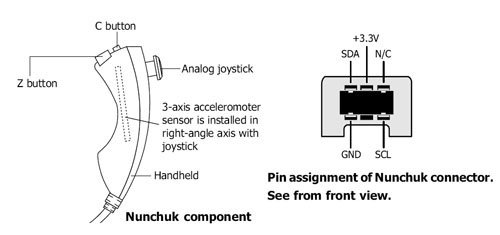
\includegraphics[width=1\linewidth]{../images/nunchuck}
		\caption[Diagrama de conexiones Wii Nunchuck]
		{Diagrama de conexiones Wii Nunchuck: observamos que contamos con las señales (SDA y SCL) y se alimenta a 3.3V  \textbf{Fuente:} \cite{nunchuck_diagram}}
		\label{fig:nunchuck}
	\end{figure}
	 
\end{itemize}


\section{Presupuesto}

En todo momento se ha tratado de optimizar el precio del desarrollo buscando componentes de reducido precio comparando entre los diferentes proveedores. Sin embargo es importante destacar que en componentes críticos (núcleo, controladora de motor) no es adecuado arriesgarse a introducir elementos de proveedores dudosos. Es por ello que se usa placa de Arduino UNO Oficial así como una controladora de motor Pololu. El desglose costes para cada componente hardware se muestra en la tabla~\ref{tabla_costes_hardware} (algunos precios pueden variar ligeramente).

\begin{table}[h!]
	\centering
	
	\begin{tabular}{|l|r|}
		\hline
		\textbf{Componente}                  				& \textbf{Precio (\euro)} \\ \hline\hline
		Arduino UNO        									&                      22 \euro \\ \hline
		Motor PaP Nema 17         							&                      10 \euro \\ \hline
		Controladora Motor (Pololu o similar) 				&                      7  \euro \\ \hline
		Pantalla LCD + controladora I2C           			&                      2.5 \euro \\ \hline
		Nunchaku Wii (compatible)        					&                      4  \euro \\ \hline
	    Sensor Temperatura, resistencias, condensador, led  & 					   1  \euro \\ \hline
		Cables, soldadura, pines, placas, etc.               &                      4  \euro \\ \hline
		Potenciómetros            							&                      2  \euro \\ \hline 
		Caja            									&                      5  \euro \\ \hline 
		Clavijas aviador            						&                      3  \euro \\ \hline 
		Fines de carrera            						&                      2  \euro \\ \hline \hline
		\textbf{Total}                  					&            \textbf{62.5 \euro} \\ \hline
	\end{tabular} 
	\caption[Lista de componentes y costes]{Lista de componentes y desglose de precios}
	\label{tabla_costes_hardware}	
\end{table}


\section{Implementación hardware}

La implementación del dispositivo hardware se puede definir como un proceso totalmente iterativo, en el marco del prototipado. Comenaremos siempre con pruebas de cada unos de los módulos por separado y trabajando con placas que permiten quitar y cambiar la distribución de los componentes.

Para realizar el diseño del circuito se utiliza la herramienta \textbf{Frizing} \cite{frizing} (figura~\ref{fig:fritzing}), de la que llama la atención su fácil uso dado que esta orientada al prototipado. Cuenta un repertorio de componentes genéricos de Arduino.

\begin{figure}[h]
	\centering
	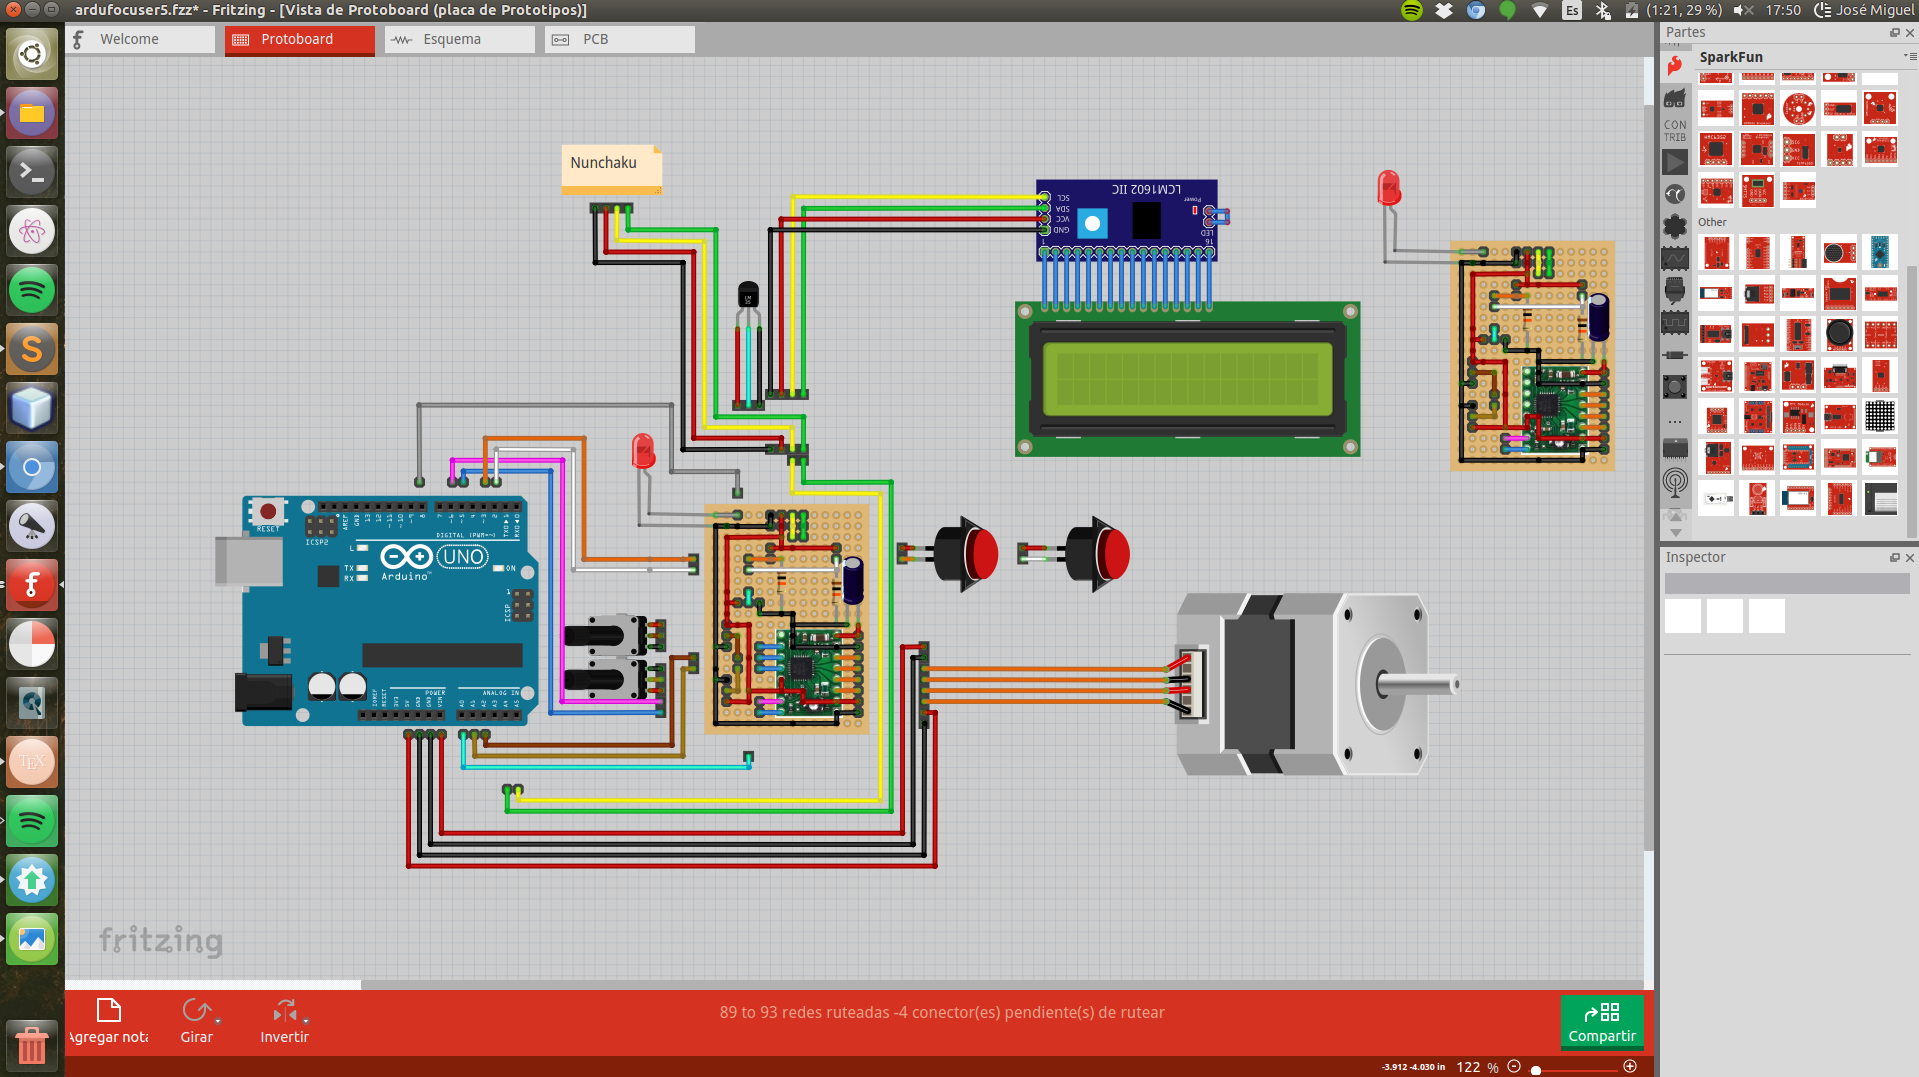
\includegraphics[width=1\linewidth]{../images/frizing}
	\caption[Diseño circuito con Frizing]{Diseño de la circuitería haciendo uso de la herramienta \textbf{Frizing}}
	\label{fig:fritzing}
\end{figure}

Una vez definido el esquemático pasamos a la fase de soldadura. Usaremos la tecnología de agujeros pasantes o \textbf{THT}, donde el circuito se monta aprovechando los orificios que trae una placa, y mediante pequeños puentes se van uniendo los agujeros creando pistas. En el diseño del circuito nos tenemos que asegurar que las pistas no se crucen (figura~\ref{fig:prototipoAgujeros}).  

\begin{figure}
	\centering
	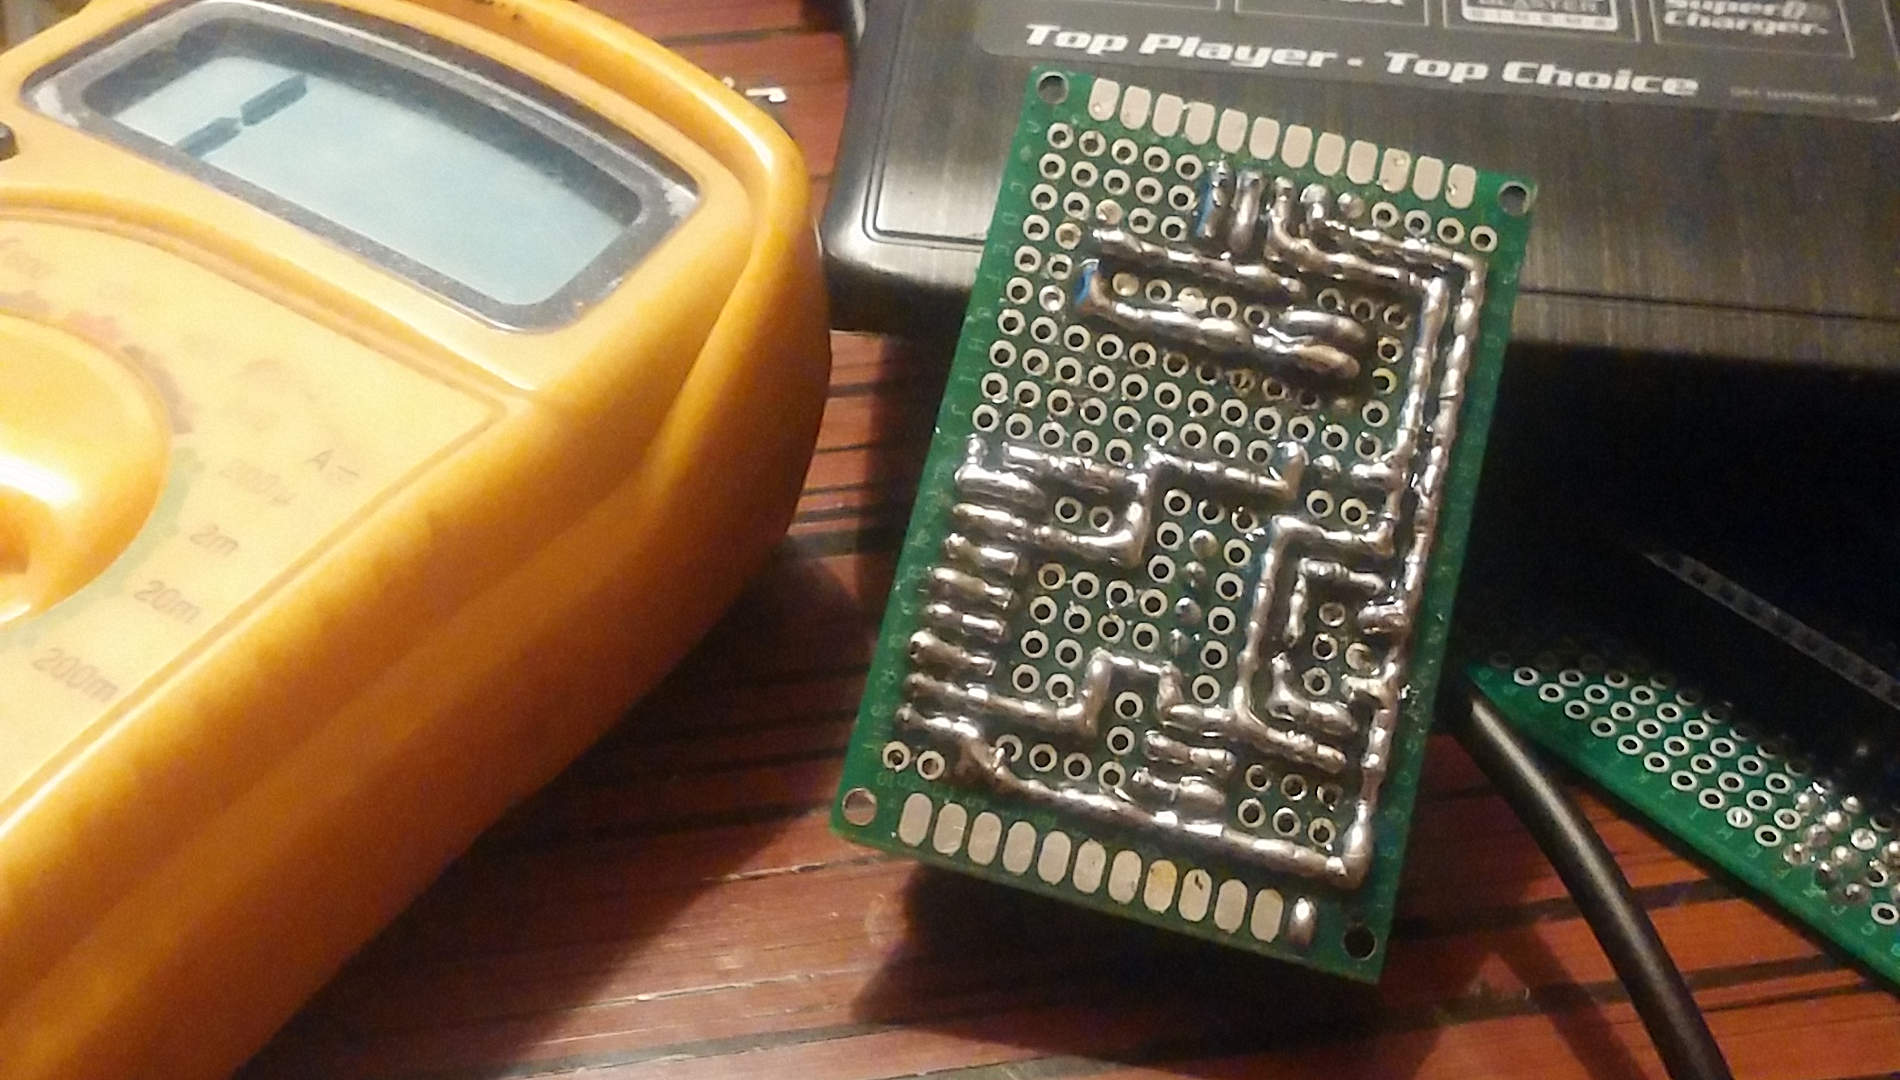
\includegraphics[width=1\linewidth]{../images/circuito01}
	\caption[Fase de soldadura de la placa]{\textbf{Fase de soldadura de la placa.} Haciendo uso de un soldador de estaño y un polimetro para comprobar continuidad, procedo a soldar un prototipo de PCB en una placa de baquelita perforada}
	\label{fig:prototipoAgujeros}
\end{figure}



\subsection{Prototipos}

Durante el proceso iterativo se han implementado cuatro versiones progresivamente más avanzadas. Detallo las características más importantes de cada uno de ellos.

\begin{itemize}
	\item \textbf{Versión 0:} Usando una placa de prototipado que permite poner y quitar los componentes sin realizar soldaduras. Se usa \textbf{LCD Keypad Shield} \cite{lcd_keypad} (figura~\ref{fig:foto_prototipo}) para reducir la dificultad inicial. LCD Keypad Shield permite utilizar una pantalla LCD y una botonera acoplándolo dicho módulo sobre Arduino MEGA. Podemos ver el diagrama seguido en la figura~\ref{circuito1} del apéndice~\ref{ap:diagramas}. 
	
	\begin{figure}
		\centering
		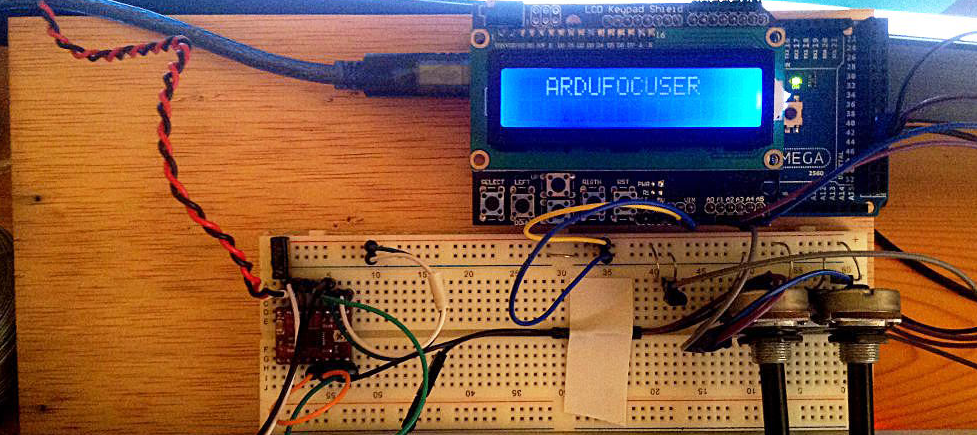
\includegraphics[width=1\linewidth]{../images/proto_recorte}
		\caption[Foto del primer prototipo]{Foto del primer prototipo, montada en placa de prototipado. Carece de carcasa y todas las conexiones se hacen usando cables.}
		\label{fig:foto_prototipo}
	\end{figure}
	
	
	\item \textbf{Versión 1:} Se realiza una completa reestructuración de los componentes, se modifica  \textbf{LCD Keypad Shield} por una pantalla LCD (interfaz de conexión clásico), una \textbf{botonera analógica} (figura~\ref{fig:botonera}) y conectores RS232 \cite{rs232}. Se puede ver el diagrama correspondiente en la figura~\ref{circuito2} del apéndice~\ref{ap:diagramas}. En la figura~\ref{fig:carcasaAluminio} se muestra la primera carcasa de aluminio realizada para el prototipo (mecanizada manualmente). Pese al buen acabado de la misma, hacen falta muchas herramientas y tiempo para construir dicha carcasa.
	
		\begin{figure}[h]
			\centering
			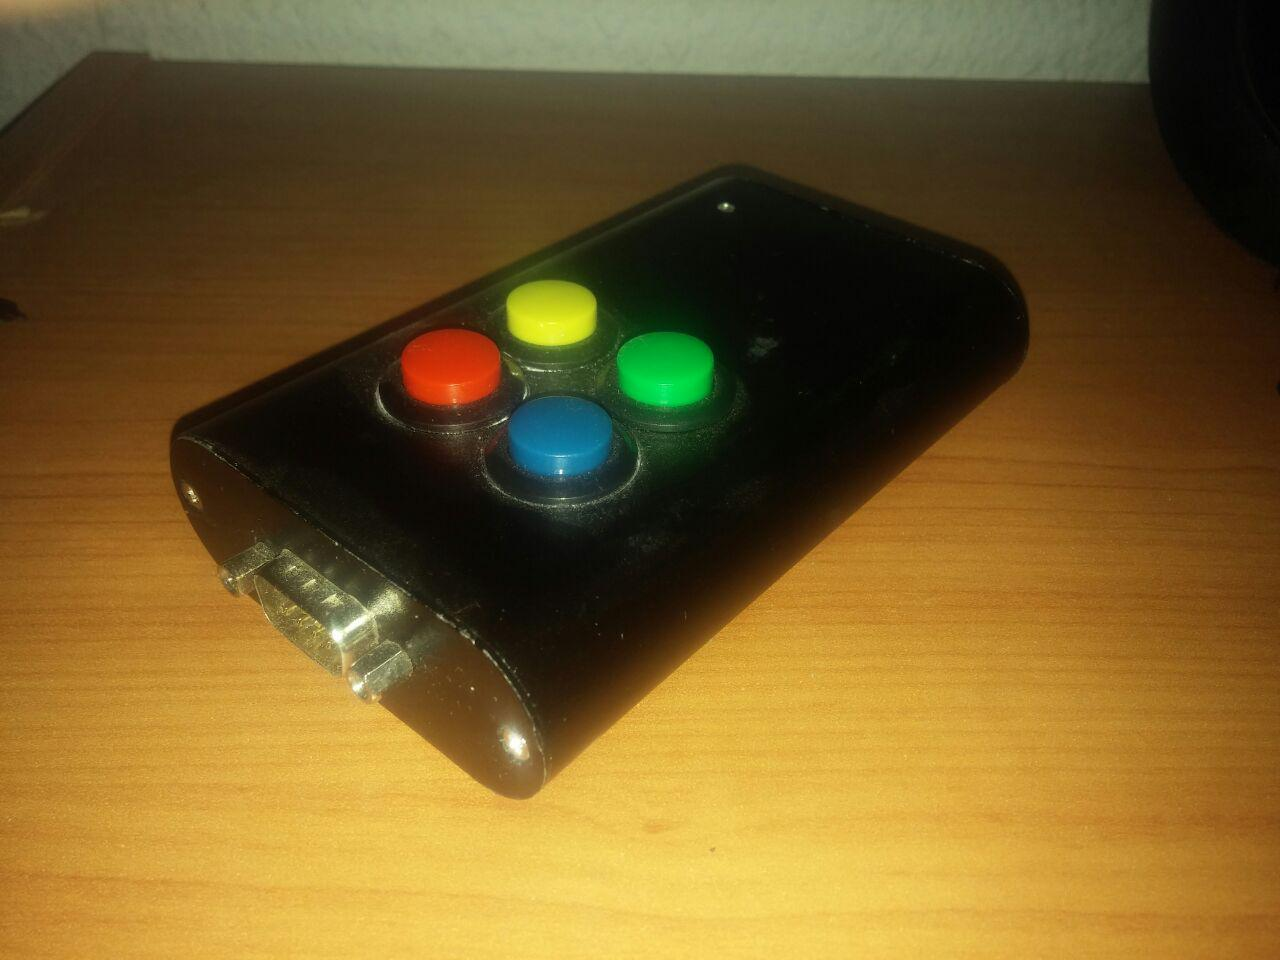
\includegraphics[width=0.75\linewidth]{../images/botonera_manual}
			\caption[Foto de la botonera manual]{Foto de la botonera manual analógica}
			\label{fig:botonera}
		\end{figure}
		
		
	\item \textbf{Versión 2:} Se rediseña modificando interfaz de la pantalla a I2C. Se intercambia la botonera manual por un mando \textbf{Wii Nunchuck} reciclado (tambien por I2C). Esto permite que se reduzca la cantidad de cables usados.  Podemos ver el circuito completo en en la figura~\ref{circuito3} del apéndice~\ref{ap:diagramas}. 
	
	\item \textbf{Versión 3:} Modificamos sensor de temperatura analógico LM35 por DHT11 (digital) (figura~\ref{circuito3} del apéndice~\ref{ap:diagramas}).
	
	\begin{figure}[h]
		\centering
		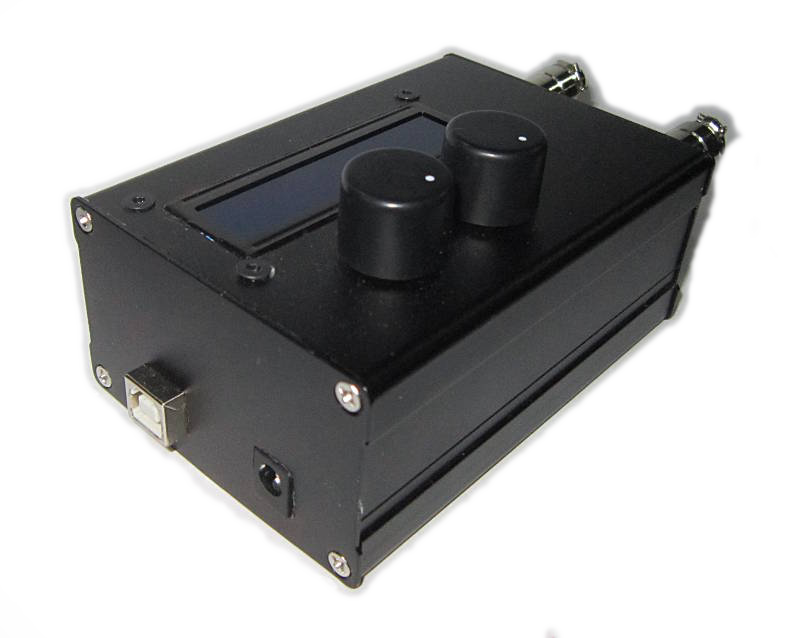
\includegraphics[width=0.9\linewidth]{../images/ardufocuser}
		\caption[Prototipo en caja de aluminio]{\textbf{Prototipo en caja de aluminio}, con un acabado muy sólido.}
		\label{fig:carcasaAluminio}
	\end{figure}
	
\end{itemize}









\section{Diseño de la carcasa y piezas mecánicas}
=======
	\item Sensor térmico: Hacemos usos de  LM35 \cite{LM35},es un sensor de temperatura con una precisión calibrada de 1 \grad C. Su rango de medición abarca desde -55 \grad C hasta 150 \grad C. La salida es lineal y cada grado Celsius equivale a 10 mV.
	\item \textbf{Bumper sensor}, o contactos fines de carrera, son interruptores todo o nada, que se activan cuando se llega a límite físico. 
\end{itemize}


\subsection{Módulo control manual}

\begin{itemize}
	\item Potenciómetros, para regular algunos valores, en concreto usamos 10 kOhms.
	
	\item Botones, para unos primeros prototipos una botonera, para activar las funciones que me interesan.
	
	\item \textbf{Wii Nunchuck}, reutilizo un mando de la consola Wii, para de una forma ergonómica activar los comandos, mediante la zeta y algunos pulsadores, este mando es totalmente compatible dado que funciona bajo el protocolo I2C.
	 
\end{itemize}

\section{Presupuesto}

\begin{itemize}
	\item Arduino UNO: 22\euro
	\item Motor PaP Nema 17: 10\euro
	\item Controladora Motor (Pololu o similar): 7\euro
	\item Pantalla LCD + controladora I2C: 2.5\euro
	\item Nunchaku Wii (compatible): 4\euro
	\item Sensor Temperatura, resistencias, condensador, led: 1\euro
	\item Cablecillos, soldadura, pines, placas, etc: 4\euro
	\item Potenciómetros: 2\euro
	\item Caja: 5\euro
	\item Clavijas aviador: 3\euro
	\item Fines de carrera: 2\euro
	
	
\end{itemize}
\textbf{Total: 62.5\euro}

\subsection{Integración de módulos}
\bigskip
Tras trabajar en cada uno de los módulos de forma independiente una visualización más o menos precisa es la siguiente:

\begin{figure}[h]
	\centering
	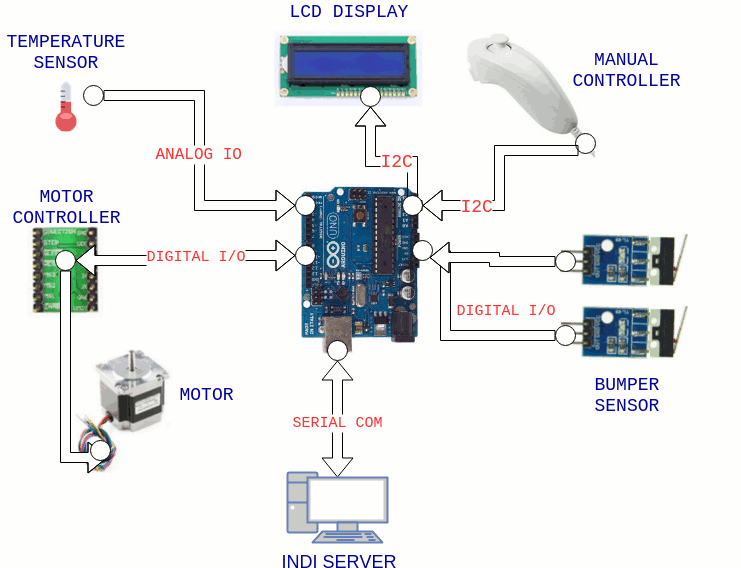
\includegraphics[width=0.9\linewidth]{../images/diagramaHardware}
	\caption{}
	\label{fig:diagramaHardware}
\end{figure}

Aún no tengo claro detalles como la alimentación de cada uno de los dispositivos,  exactamente las conexiones que va a requerir cada periférico ni su ubicación.

\bigskip
Es importante contabilizar número de pines que necesita cada periférico, si son digitales o analógico, pwd o hacen uso de interrupciones hardware. 

\bigskip
Con ello nos podemos hacer una idea aproximada del sistema y de los recursos que necesitamos.


\newpage
\section{Implementación hardware}

La implementación del dispositivo hardware, se puede definir como un proceso totalmente iterativo, en el marco del prototipado, comenzando por las pruebas de cada unos de los módulos, y trabajando con placas que permiten remover y cambiar la distribución de los componentes.



\begin{figure}[h]
\centering
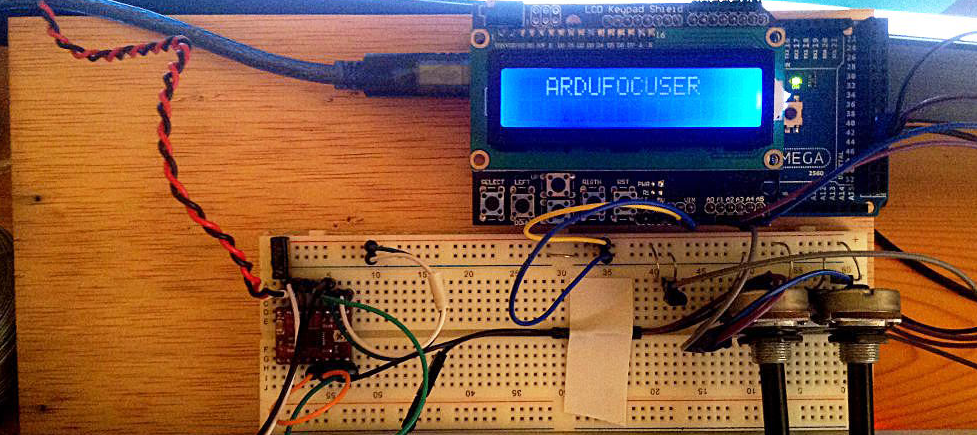
\includegraphics[width=0.7\linewidth]{../images/proto_recorte}
\caption{}
\label{fig:prototipoArdufocuser}
\end{figure}

\bigskip
Tras muchas pruebas y una vez claras las partes fundamentales de las que consta el dispositivo, así como su integración, se pasa a formalizar el diseño, buscando la elegancia, la máxima limpieza en la distribución de los componentes, así como la economía de espacio.

\begin{figure}[h]
	\centering
	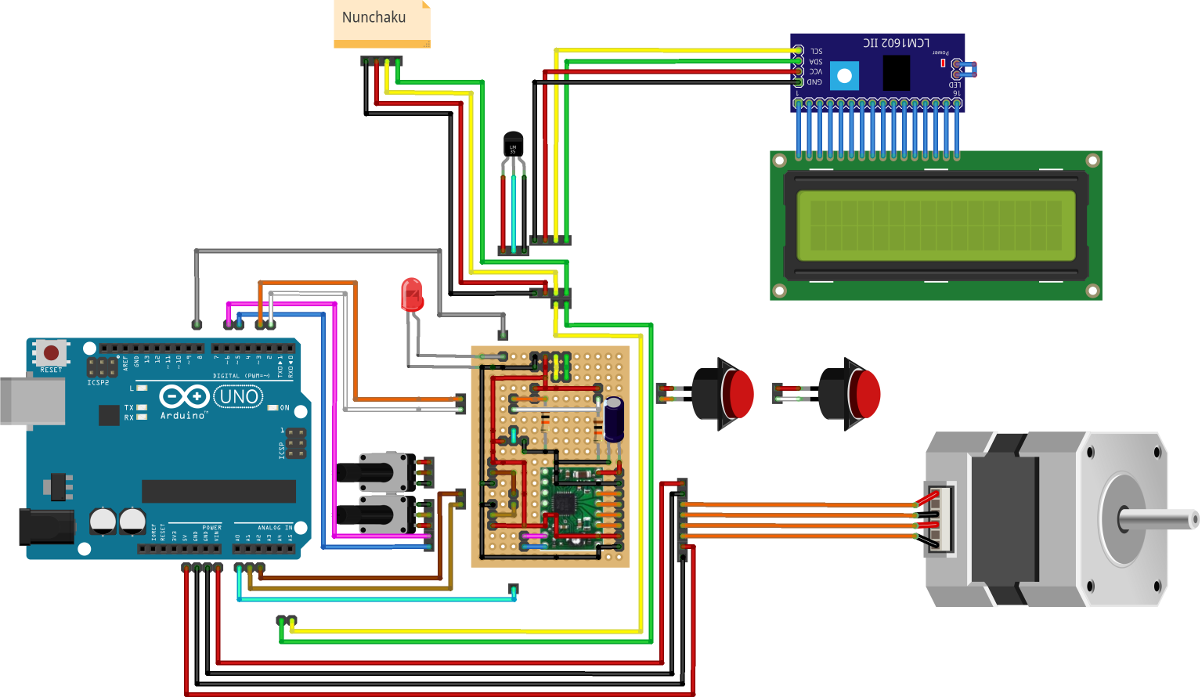
\includegraphics[width=1\linewidth]{../images/circuito}
	\caption{}
	\label{fig:prototipoArdufocuser}
\end{figure}


Una vez perfectamente definido el esquemático pasamos a la fase de soldadura.

\newpage


\section{Diseño carcasa y piezas mecánicas}
>>>>>>> c9f08dfe66521d4f0dba18e652f93a6a37a333aa

Para dar soporte a toda la electrónica, así como hacer el dispositivo robusto y fácilmente transportable,
se decide diseñar una carcasa que permita cubrir toda la electrónica y concentrar todos los conectores y botones. 

<<<<<<< HEAD
Para ello debemos hacer una buena estimación del espacio y la distribución de los elementos. Otro punto a tener en cuenta es que debemos permitir la fácil apertura y manipulación del los elementos internos, con el fin de poder realizar mejoras o simplemente permitir a los interesados abrir el dispositivo y conocer sus interioridades. 

En un primer momento se optó por adquirir cajas prefabricadas a un proveedor externo y se estudiaron diferentes diseños.


El acabado era excelente, pero se encontraron varios inconvenientes:

\begin{itemize}
	\item \textbf{Dependencia de un proveedor}, que facilite siempre el mismo modelo de caja.
	\item \textbf{Diseño poco personalizable}, debemos asegurarnos de que el dispositivo se adapte perfectamente a las dimensiones.
	\item  \textbf{Difícil mecanización}, dado el material metálico, realizar agujeros pasantes, soldaduras, grabados, roscas etc, se convierte en tareas tediosas. 
\end{itemize}

Por estos motivos decidimos plantear la alternativa de fabricar una carcasa propia. Dado que contamos con una \textbf{cortadora láser} controlada numéricamente decidimos crear una carcasa totalmente propia a partir de laminas de \textbf{metacrilato} de 3mm de espesor (figura~\ref{fig:cajaMetacrilato}).

\begin{figure}
	\centering
	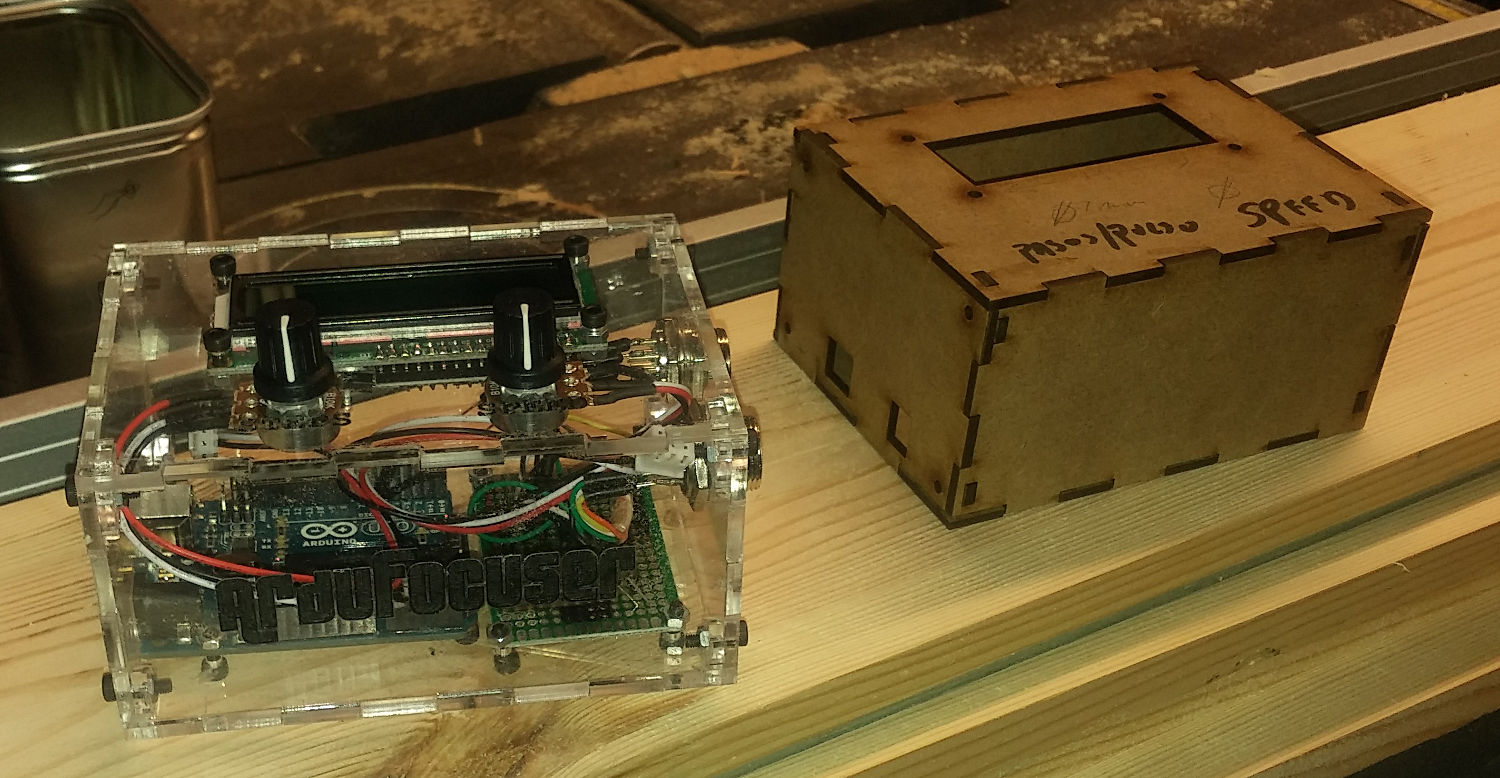
\includegraphics[width=1\linewidth]{../images/cajas}
	\caption[Foto de la carcasa en metacrilato]{\textbf{Resultado después del corte de la carcasa en metacrilato}. Previamente se realizan ensayos en materiales más baratos como \textbf{DM} \cite{dm}.}
	\label{fig:cajaMetacrilato}
\end{figure}
=======
Para ello debemos hacer una buena estimación del espacio y la distribución de los elementos, otro punto a tener en cuenta es que debemos permitir la fácil apertura y manipulación del los elementos internos, con el fin de poder realizar mejoras o simplemente permitir a los interesados abrir el dispositivo y conocer sus interioridades. 

En un primer momento se optó por adquirir cajas prefabricadas a un proveedor externo y estudié diferentes diseños.

\begin{figure}
\centering
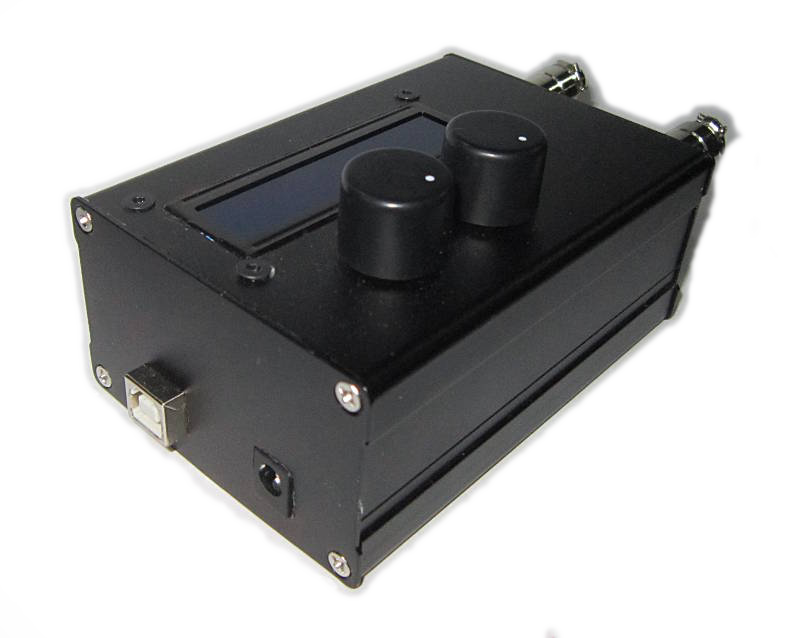
\includegraphics[width=0.7\linewidth]{../images/ardufocuser}
\caption{}
\label{fig:ardufocuser}
\end{figure}


El acabado era excelente, pero me encontraba varios inconvenientes, por los cueles decidí plantearme la alternativa de fabricar mi propia carcasa "Ardufocuser". 

\begin{itemize}
	\item Dependencia de contar con un proveedor que facilite siempre el mismo modelo de caja.
	\item Diseño poco personalizable, debo asegurarme que el dispositivo se adapte perfectamente a las dimensiones.
	\item  Difícil mecanización, dado el material metálico, realizar agujeros pasantes, soldaduras, grabados, roscas etc, se convertían en tareas tediosas. 
\end{itemize}

Dado que contamos con una cortadora láser de última generación decidimos, crear una carcasa totalmente propia, a partir de laminas de "metacrilato".
>>>>>>> c9f08dfe66521d4f0dba18e652f93a6a37a333aa

Ventajas de esta opción:

\begin{itemize}
	\item Bajo coste de los materiales. 
	\item Totalmente personalizada y a medida.
<<<<<<< HEAD
	\item Replicable al 100\%.
\end{itemize}

En el apéndice~\ref{ap:caja} se muestran algunas imágenes del diseño de la caja con un programa de modelado 3D así como los el fichero SVG con los planos de las piezas utilizado para el corte de la misma.


\section{Pruebas sobre el dispositivo hardware}

La sección de pruebas las dividimos en varias partes, pasando pruebas de concepto de cada uno de los componentes y módulos individuales, pruebas de integración, pruebas de rendimiento. 

\begin{itemize}
	\item \textbf{Pruebas de concepto y de componentes:} Es necesario revisar que los componentes que hemos adquirido no tienen ningún defecto que de ser detectados más adelante pueden ser costosos de cambiar. En las tablas~\ref{tab:prueba1},~\ref{tab:prueba2} y ~\ref{tab:prueba3} se muestran algunos de los casos de prueba realizados. 
	
	\begin{table}[h]
		\centering

		\begin{tabular}{|l|l|}
			\hline
			ID caso de prueba             &  1 \\ \hline
			Nombre prueba                 &  Prueba lectura potenciómetros \\ \hline
			Autor de la prueba            &  José Miguel López \\ \hline
			Responsable diseño            &  José Miguel López \\ \hline
			Pasos y condiciones ejecución &  \begin{tabular}[c]{@{}l@{}}
													- Compilar y cargar sketch (\ref{lst:potenciometro_test_code})\\
													- Conectar placa a la alimentación \\
													- Variar resistencia en los potenciómetros.							
											 \end{tabular} \\ \hline
			Resultado deseado             & \begin{tabular}[c]{@{}l@{}}
											Se debe pintar por pantalla valores \\
											de 0 a 100 proporcionales a la resistencia. \\
										\end{tabular} \\ \hline
		
			Resultado obtenido            &  \begin{tabular}[c]{@{}l@{}}
												Se pintan por pantalla valores \\
												de 0 a 100 proporcionales a la resistencia. \\
										     \end{tabular} \\ \hline
			
			Estado caso de prueba         &  Éxito\\ \hline
			Errores asociados             &  Ninguno\\ \hline
			Comentario                    &  \\ \hline
		\end{tabular}
				\caption{Caso de prueba, lectura de potenciómetros}
		\label{tab:prueba1}
	\end{table} 
	
	
	\begin{table}[h]
		\centering

		\begin{tabular}{|l|l|}
			\hline
			ID caso de prueba             &  2 \\ \hline
			Nombre prueba                 &  Prueba mover motor velocidad constante \\ \hline
			Autor de la prueba            &  José Miguel López \\ \hline
			Responsable diseño            &  José Miguel López \\ \hline
			Pasos y condiciones ejecución &  \begin{tabular}[c]{@{}l@{}}
				- Compilar y cargar sketch (\ref{lst:motor_test_code})\\
				- Conectar placa a la alimentación \\						
			\end{tabular} \\ \hline
			Resultado deseado             & \begin{tabular}[c]{@{}l@{}}
				El motor debe girar a velocidad constante \\ y de forma uniforme.
			\end{tabular} \\ \hline
			
			Resultado obtenido            &  \begin{tabular}[c]{@{}l@{}}
				El motor gira a velocidad constante y de \\ forma uniforme.
			\end{tabular} \\ \hline
			Estado caso de prueba         &  Éxito\\ \hline
			Errores asociados             &  Ninguno\\ \hline
			Comentario                    &  \\ \hline
		\end{tabular}
				\caption{Caso de prueba, mover motor a velocidad constante}
		\label{tab:prueba2}
	\end{table} 
	
	
	\begin{table}[h]
		\centering

		\begin{tabular}{|l|l|}
			\hline
			ID caso de prueba             &  3 \\ \hline
			Nombre prueba                 &  Prueba mando Nunchuck \\ \hline
			Autor de la prueba            &  José Miguel López \\ \hline
			Responsable diseño            &  José Miguel López \\ \hline
			Pasos y condiciones ejecución &  \begin{tabular}[c]{@{}l@{}}
												- Compilar y cargar sketch (\ref{lst:nunchuck_test_code})\\
												- Conectar placa a la alimentación \\
												- Pulsar sobre los diferentes botones del mando.						
											\end{tabular} \\ \hline
			Resultado deseado             & \begin{tabular}[c]{@{}l@{}}
												Se debe pintar en la pantalla LCD: \\
												- LEFT: Cuando movemos la palanca \\hacia la izquierda.\\
												- RIGHT: Cuando movemos la palanca \\hacia la derecha.\\
												- Z: Al pulsar el botón Z.\\
												- C: Al pulsar el botón C.\\
											\end{tabular} \\ \hline
											
			Resultado obtenido             & \begin{tabular}[c]{@{}l@{}}
				Se pinta en la pantalla LCD: \\
				- LEFT: Cuando movemos la palanca \\ hacia la izquierda.\\
				- RIGHT: Cuando movemos la palanca \\ hacia la derecha.\\
				- Z: Al pulsar el botón Z.\\
				- C: Al pulsar el botón C.\\
			\end{tabular} \\ \hline
			Estado caso de prueba         &  Éxito\\ \hline
			Errores asociados             &  Ninguno\\ \hline
			Comentario                    &  \\ \hline
		\end{tabular}
				\caption{Caso de prueba, detectar pulsaciones en Wii Nunchuck}
		\label{tab:prueba3}
	\end{table} 
	
		   
	\item \textbf{Pruebas de rendimiento:} Comprobar que el sistema es tolerante a fatigas, no se sobrecalienta ningún componente y continua siendo estable  después de un tiempo prolongado. En la tabla~\ref{tab:prueba4} se muestran uno de los casos de prueba realizados. 
	
	
		\begin{table}[h]
			\centering

			\begin{tabular}{|l|l|}
				\hline
				ID caso de prueba             &  4 \\ \hline
				Nombre prueba                 &  Prueba temperatura motor \\ \hline
				Autor de la prueba            &  José Miguel López \\ \hline
				Responsable diseño            &  José Miguel López \\ \hline
				Pasos y condiciones ejecución &  \begin{tabular}[c]{@{}l@{}}
					- Compilar y cargar sketch (\ref{lst:motor_test_code})\\
					- Conectar placa a la alimentación \\
					- Dejar el circuito conectado durante 120 minutos.					
				\end{tabular} \\ \hline
				Resultado deseado             & \begin{tabular}[c]{@{}l@{}}
					La temperatura del motor debe ser normal \\
					no debe existir sobrecalentamiento.
				\end{tabular} \\ \hline
				
				Resultado obtenido            &  \begin{tabular}[c]{@{}l@{}}
					El motor presenta una temperatura \\ por encima de la normal \\
				\end{tabular} \\ \hline
				Estado caso de prueba         &  Error \\ \hline
				Errores asociados             &  Se puede quemar el motor con un uso más prolongado. \\ \hline
				Comentario                    &   \begin{tabular}[c]{@{}l@{}}
													Se diagnostica posible causa, \\
													 mal reglaje en la alimentación del motor. 
											\end{tabular} \\ \hline
			\end{tabular}
						\caption{Caso de prueba, temperatura de motor tras un tiempo de funcionamiento prolongado}
			\label{tab:prueba4}
		\end{table} 
\end{itemize}





=======
	\item  Replicable 100\textdiscount
\end{itemize}


% Meter foto caja metacrilato.


\section{Pruebas sobre el dispositivo hardware.}


La sección de pruebas las dividimos en varias partes, pruebas de concepto de cada uno de los componentes y módulos individuales, pruebas de integración, pruebas de rendimiento. 




\begin{figure}[h]
\centering
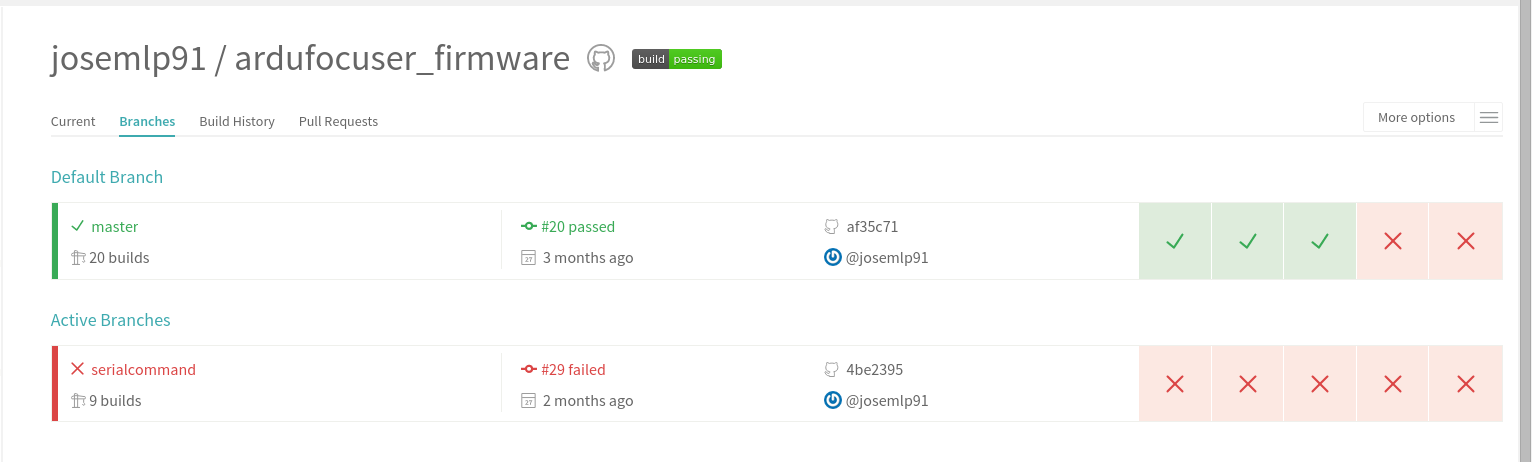
\includegraphics[width=1\linewidth]{../images/travis_ci}
\caption{}
\label{fig:travis_ci}
\end{figure}

\begin{figure}[h]
	\centering
	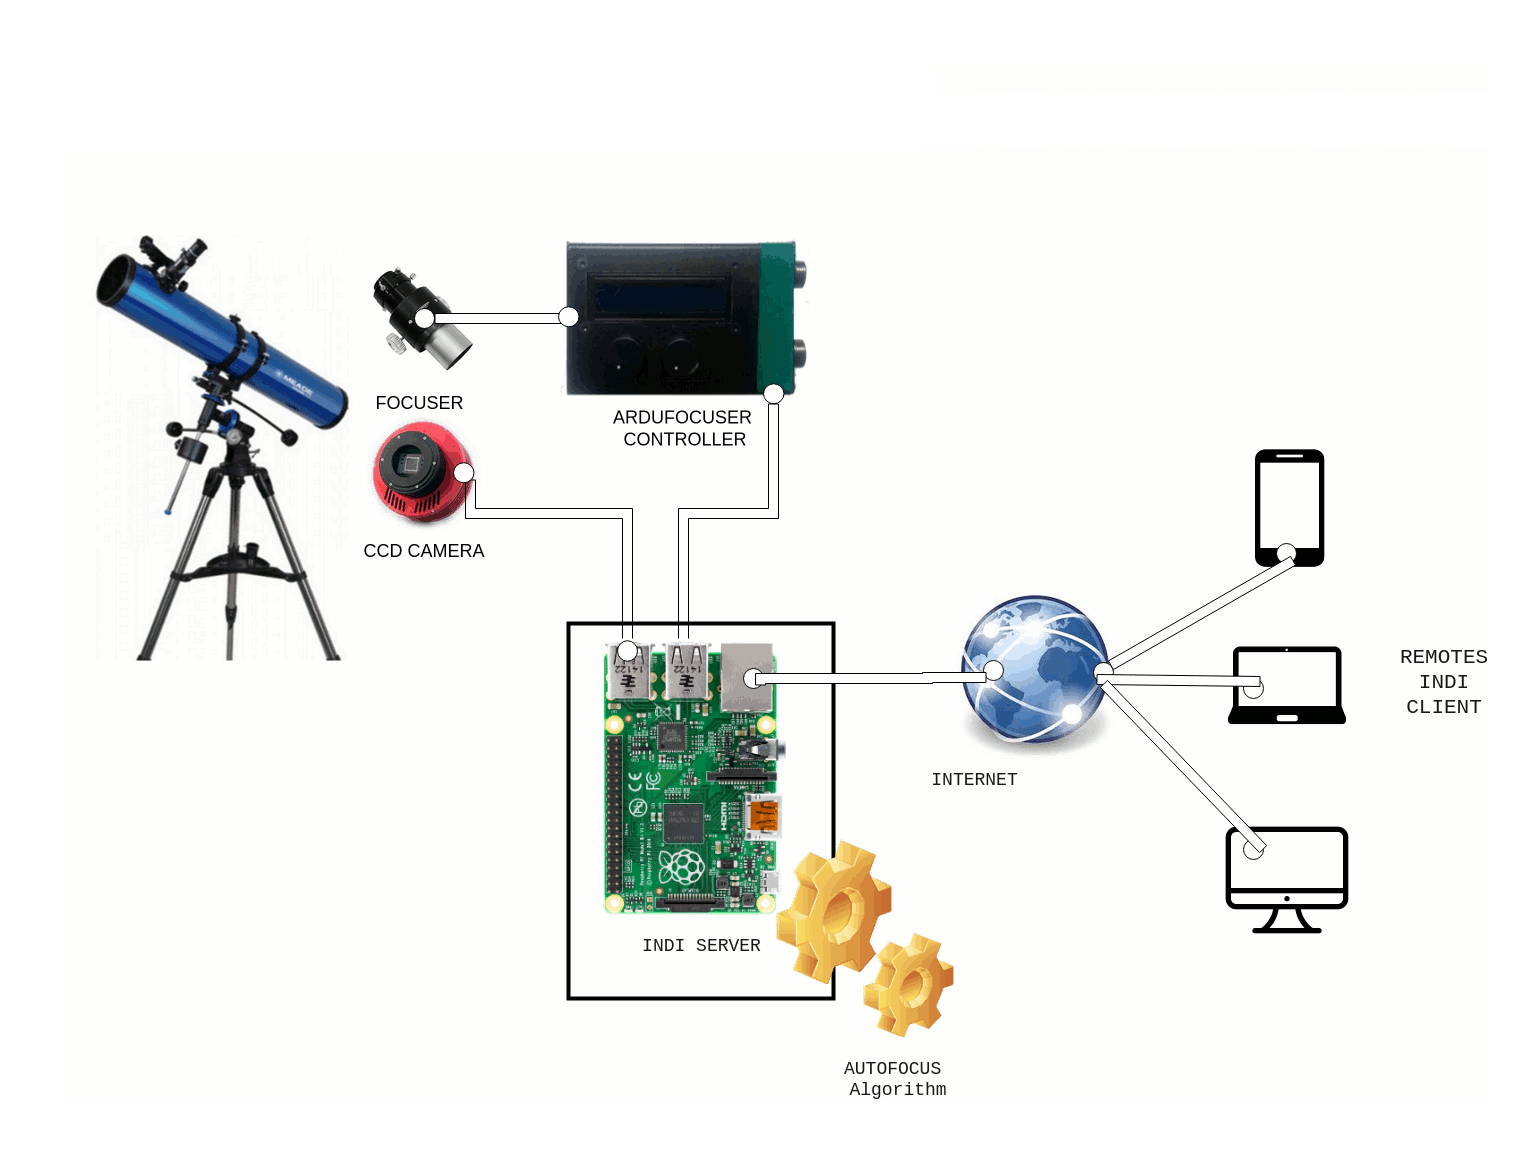
\includegraphics[width=0.7\linewidth]{../images/diagramaGeneral}
	\caption{}
	\label{fig:diagramaHardware}
\end{figure}


\begin{figure}[h]
	\centering
	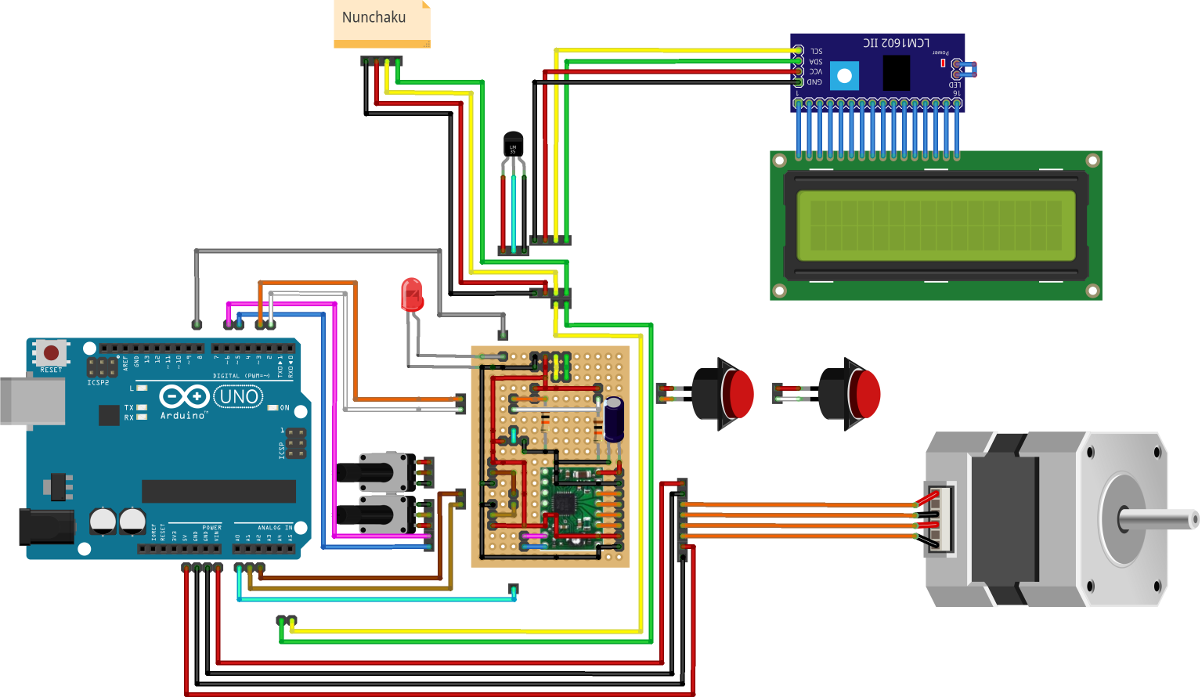
\includegraphics[width=0.7\linewidth]{../images/circuito}
	\caption{}
	\label{fig:diagramaHardware}
\end{figure}
>>>>>>> c9f08dfe66521d4f0dba18e652f93a6a37a333aa


